%!TEX root = ../Thesis.tex
\chapter{Discussion and outlook}
\label{sec:discussion}

%--------------------------------------------------------------------------------
\clearpage
\section{What remote sensing can be used for in the context of minute-scale wind forecasting}
\label{sec:discussion_rs}
\bigskip

Two approaches to remote sensing based forecasting have been demonstrated in this thesis work which indicate the usefulness of such a system.

The first is predicting the wind speed and direction minutes-ahead using upwind radial speed measurements together with a propagation model. The second is using the upwind observations to detect and track coherent structures advecting towards the site. These can include events such as weather fronts and wind ramps.

Various applications of operational forecasts on these timescales (i.e 0-60 minutes) have been identified, including the following:

\begin{itemize}
    \item Wind farm control including induction control and wake steering/deflection.
    \item Trading in electricity markets with lead times below one-hour. Present day examples include Australia, and the EPEX Spot markets for national trades within Germany, France, Austria, Switzerland, Belgium and the Netherlands.
    \item Power grid balancing for voltage and frequency control by TSOs. This includes reserve capacity and regulating actions through ancillary service markets which are presently operating in the Spanish and German grids using wind power plants.
    \item Asset management by wind power owners and operators, including portfolio optimization and storage (e.g. battery) control.
\end{itemize}

Site measurements from remote sensing devices offer high-resolution information about local conditions which dominate the minute-scale wind variability. As the wind is fundamentally chaotic, it is arguable that numerical weather prediction (NWP) models on their own will continue to struggle considerably in the lasting future to correctly resolve these microscale turbulence features. Boundary conditions used for initializing NWP models may originate from remote sensing devices like Doppler lidar or radar (i.e. data assimilation), but present computational resources do not enable results to be available fast enough for real time operation on the minute scale.

In contrast, all forecast methods demonstrated in this body of work are capable of real time use. However it remains to be answered if any skill increase towards reducing forecast errors can be capitalized upon by the wind power industry. The lidar instrumentation used in the field experiments must be purchased, installed and maintained by skilled technical staff to provide accurate and reliable measurement data. These additional capital and operational expenses may not translate into a net benefit when compared with 'free' methods which use only existing data sources. That being said, as remote sensing device manufacturers mature and compete to improve product cost, and large wind farms approach and exceed the gigawatt scale of installed capacity, the business case for installing and operating such a system may become feasible as even very small gains can result in significant economic impacts.

Within the minute-scale, all proposed methods must be benchmarked against statistical time series modelling approaches such as ARIMA which in surprisingly many cases outperforms the more complex lidar based methods examined here. The question as to whether or not ARIMA approaches can be consistently beaten using lidar propagation models also remains unanswered. The greatest opportunities for constructive impacts seem to lie in using the lidar system for detecting and tracking anomalies, either through a pure data driven approach or in a hybrid manner with existing NWP models. Although partly investigated, this was not the main theme addressed in the PhD project.

%--------------------------------------------------------------------------------
\clearpage
\section{Recommended practical implementations}
\label{sec:discussion_practical}

In this section, a number of practical suggestions are made towards an operational realization of a lidar based forecasting system.

Current commercially available pulsed scanning lidar systems are suitable tools, but are designed with excessive capabilities relative to the design requirements of propagation based and extreme event detection forecasting methods. Significant application specific simplifications can be made which would increase the robustness and reliability of the instruments as well as decrease their cost and maintenance demands. Fixed beam formulations similar to existing nacelle lidar models could be adapted for this purpose by increasing the power of the laser source and fibre amplifiers to achieve measurement ranges equal to the high-power scanning variants.

The significant added cost, complexity, and reliance on concurrent data availability using multiple systems in dual or triple Doppler configurations leads to the recommendation for deploying single units to scan at each region of interest upstream, and for obtaining wind field information either using the radial speed measurements directly, or through SDVR post-processing techniques to obtain the reconstructed horizontal wind vector components.

The field experiments have utilized two versions of publicly available scanning lidar hardware- the Leosphere Windcube 200S and 400S. The 400S has an expanded measurement range compared to the 200S system, and is preferred for this application in order to provide increased data availability at further distances. Ultimately, the scanning geometry of the WAFFLE experiment where the 400S was used led to a lack of success in capitalizing on the increased range. This was due to the ground based deployment where the instrument was not scanning horizontally. The experiments have also taught us that for feature tracking, it is preferable to trade detail (spatial resolution) for a higher scan rate (temporal resolution). The coherent structures naturally morph and transform as they advect. Increasing the scan rate allows for improved tracking, in addition to reducing distortion of the features due to the fact that the scans are not an instantaneous snapshot in time.

Although all field experiments performed during the project took place onshore, they have all attempted to emulate offshore conditions as much as possible (i.e. by reducing the effects of surface roughness and taking place in coastal environments). This is the recommended direction for any real world realization of such a system. The increased turbulence from terrain and surface effects, together with the possibility to deploy cheaper and simpler ground based instruments (e.g. masts and profiling lidars) around the site makes the idea better suited for the constraints of offshore locations.

A proposed framework for operating at a wind farm would be to install a simplified turbine mounted device within the first and/or last row (see Fig. \ref{fig:discussion_layout}), or several devices placed at the corners of the turbine array to provide spatial coverage for all wind directions. Mounting the device at close to hub height (either atop the nacelle or fixed to the tower) will ensure that the horizontal wind measurements are not affected by wind shear or vertical wind motion (a lesson learned during the WAFFLE campaign). Similarly to traditional nacelle lidars, beam blockage by the turbine blades and tilting from trust loading of the rotor and structure are necessary considerations. An alternative setup would be to deploy a traditional ground based or tower mounted scanning lidar (onshore) or atop a substation platform in offshore environments. In this configuration, the scanning lidar would perform either continuous 360\degree \ PPI scans, or would perform an initial calibrating sector scan to determine the general wind direction, and then launch repeating scans centered in that direction. 

\begin{figure}[htbp]
    \centering
        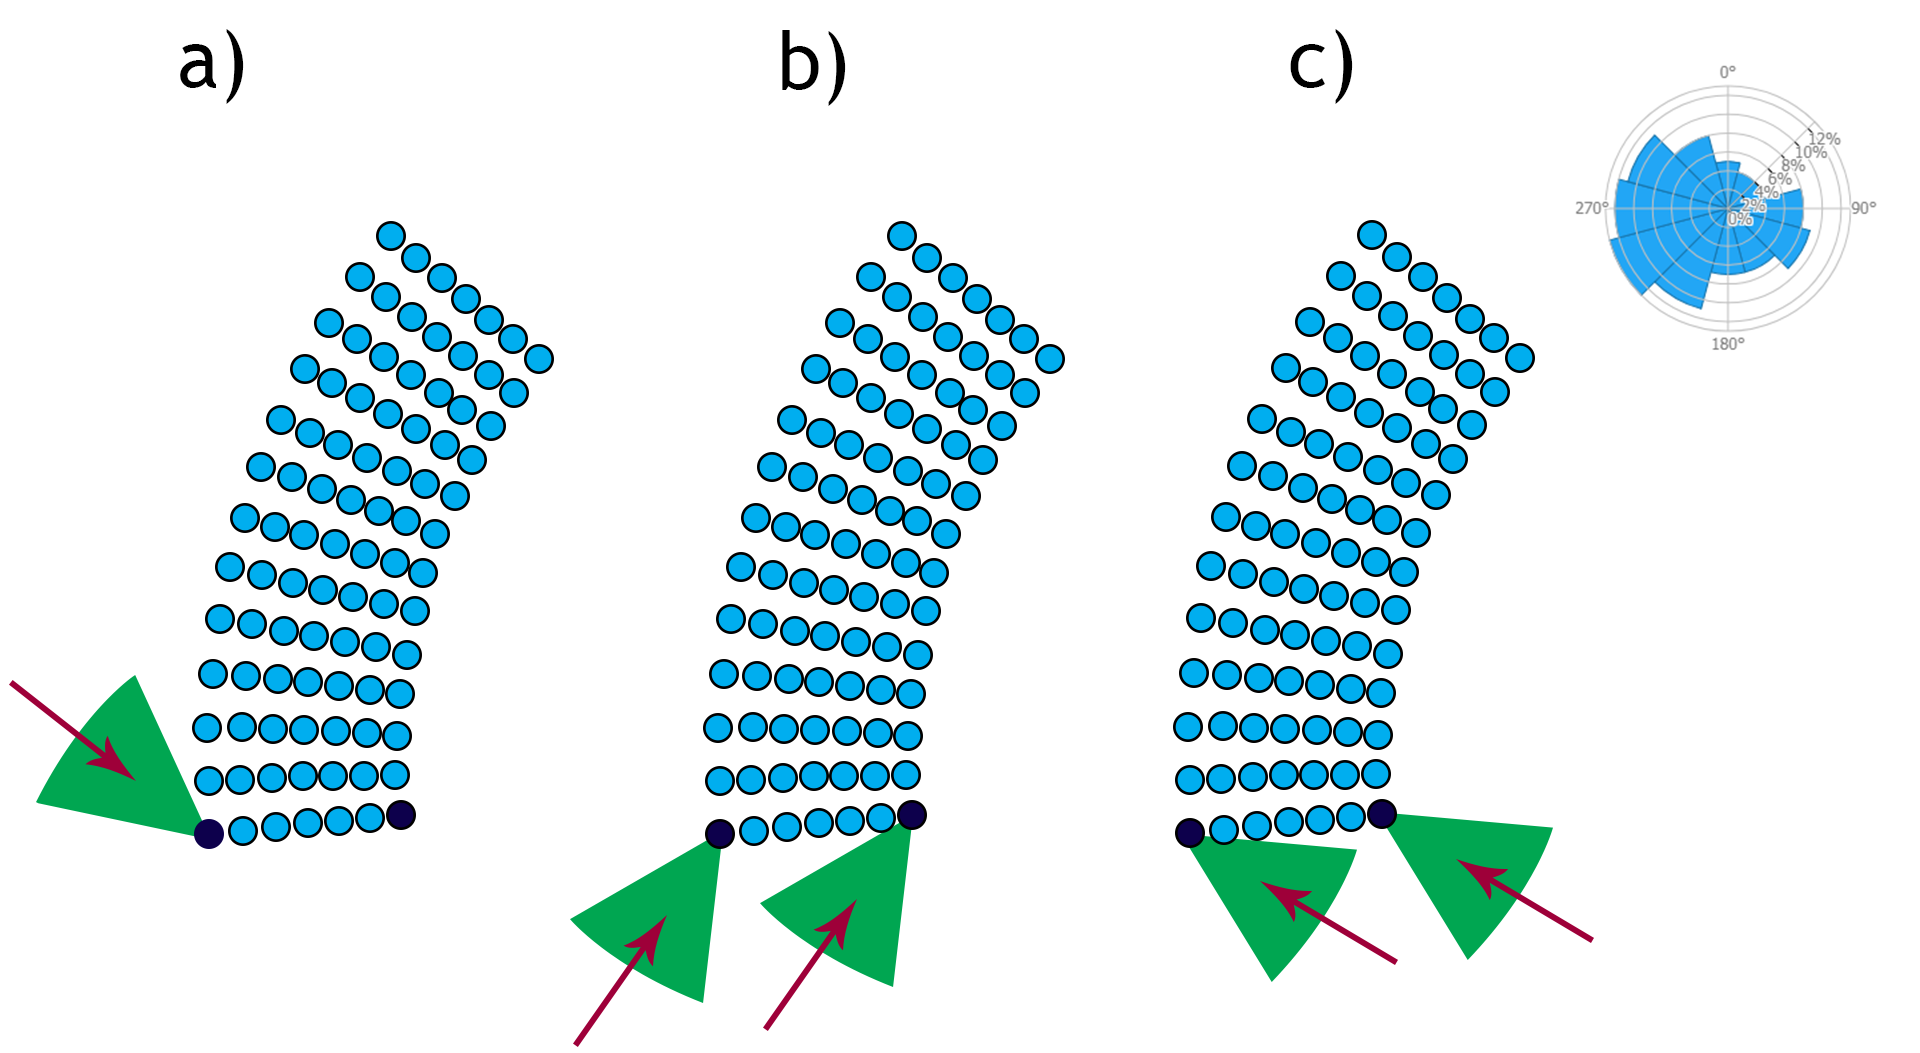
\includegraphics[width=0.8\textwidth]{graphics/discussion_layout.png}
    \caption{An example of a conceived operational system at the Horns Rev 2 offshore wind farm. The wind rose is shown in the top right corner, with data obtained using the Global Wind Atlas. Two lidar systems are mounted on the dark blue turbines and measure within a given angular width of the presiding wind direction (indicated with red arrows). This allows for coverage of the predominant climatology at the site: NW to SW winds (a-b), and S to E winds (c)}
    \label{fig:discussion_layout}
\end{figure}

When processing measurement data, it is recommended to utilize advanced filtering techniques such as the dynamic method (\cite{beck_dynamic_2017}) instead of a strict threshold filter to increase the effective measurement range. In cases where the lidar device does not provide sufficient data quality, a fall back approach should be included which instead relies of the persistence method within the first 30-seconds, and ARIMA time series modelling after that horizon. The level of sophistication required for processing lidar PPI measurements is lower for wind speed than direction. In the case of wind speed, the simple maximum-absolute-magnitude retrieval method is sufficient. However the high sensitivity and low resolution of this method for wind direction retrieval makes it ill advised. In cases of needing accurate wind direction information, it is preferable to apply fitting algorithms such as IVAP.

In regards to forecast model formulation, two separate approaches are reviewed. The first being event detection, either for extreme events or for anticipated situations predicted by NWP models (i.e. a hybrid approach). This method utilizes real time measurements together with a static set of rules (i.e. model) to determine if an event is detected within close proximity to the site. Examples include monitoring the upstream wind speed or direction gradient to detect approaching weather regimes changes, or other highly localized meteorological phenomena. This is formulated as a classification problem and as such does not require any past information being time-independent by design. This method can however be optionally combined with a spatiotemporal advection model to predict the arrival timing of the event.

The second approach is based either on a simple time of flight shifting of upwind measurements, or on regression models which employ real time spatiotemporal correlations to predict wind vectors minutes-ahead. Due to the high temporal autocorrelation of the wind signals and the short stability of atmospheric conditions, model weights in the latter approach should be tuned as close to real time as possible. This can be done be incrementally re-fitting the existing model with new observations as they become available, or by training a new model on a rolling window of past observations or on the entire dataset at each timestep. It is also recommended to generate forecasts in a multi-output fashion (i.e. a vector forecast spanning a range of lead times) to ensure that all space time correlations can be extrapolated into the forecast.

%--------------------------------------------------------------------------------
\clearpage
\section{Opportunities for extension of work}
\label{sec:discussion_extension}

The limited duration of this project has imposed limits on the scope of the research and field work carried out. For future work on the subject, a number of possible continuations are suggested together with the open-ended questions presented earlier in this discussion section.

All forecasts in this body of work have been deterministic (single point predictions). Probabilistic forecasts are emerging as the new standard as they also contribute information about the range and distribution of uncertainties around the predicted values. This is useful for modelling sensitivities and in decision making, e.g. applying optimal bidding strategies to minimize risk when participating in the auction markets (\cite{pinson_trading_2007}). Outputs from multiple deterministic models can be transformed into prediction intervals by methods including quantile regression averaging (\cite{nowotarski_computing_2015}), support vector quantile regression (\cite{he_short-term_2017}), or approaches based on logistic regression.

As discussed in Section \ref{sec:discussion_practical}, a suggestion for future field measurements is to define an adaptive scan trajectory which tracks the general wind direction, instead of repeating a fixed pattern which may not be focused upwind of the site. Other continuations of the measurement efforts include trials with large-scale Doppler lidars such as the Lockheed Martin WindTracer or Mitsubishi Diabrezza A which can measure at distances up to 30 km for increased look-ahead time. It is also suggested to explore beyond flat cross sections of the horizontal wind, by including e.g. vertical cross sections from RHI scans, or even 3-D volumetric trajectories to account for wind shear and the vertical structure of atmospheric motion.

State of the art wind farm models (e.g. PossPOW from DTU) have been recently applied for second-scale forecasting, using SCADA signals from within the wind farm to predict power production at downstream turbine rows during periods of normal and down-regulated operation (\cite{gocmen_possible_2019}). This system is envisioned to eventually interface with an operational wind farm controller and also enable grid support in the form of reserve power provisions. A coupling between one of the approaches outlined in this thesis which predicts for the first row, together with a wind farm model for the remaining turbines presents a natural combination which should be explored in future work.

\begin{comment}
Extension of work:
What we still don't know
tune ANN model
When does ARIMA fail?
\end{comment}